\documentclass[tikz,border=12pt]{standalone}
\usepackage[T1]{fontenc}
\usepackage{helvet}
\renewcommand{\familydefault}{\sfdefault}
\usepackage{amsmath}
\usetikzlibrary{arrows.meta, fit, backgrounds, positioning, calc, shapes.geometric}

% Semantic palette: teal = dense / neural step; gray = neutral glue;
% amber = stores; (no green output here, indexing ends in a store).
\definecolor{queryfill}{HTML}{ECEFF2}
\definecolor{queryborder}{HTML}{8A96A3}
\definecolor{encfill}{HTML}{DCEFE9}
\definecolor{encborder}{HTML}{2E9478}
\definecolor{corpusfill}{HTML}{FBF0D5}
\definecolor{corpusborder}{HTML}{CFA23E}
\definecolor{regfill}{HTML}{F6F8FB}
\definecolor{regborder}{HTML}{C4CDD6}
\definecolor{darkline}{HTML}{333333}
\definecolor{subtext}{HTML}{5A5A5A}

\tikzset{
  card/.style={rectangle, rounded corners=5pt, align=center, draw=darkline,
               line width=0.8pt, minimum height=1.2cm, font=\small},
  glue/.style={card, fill=queryfill, draw=queryborder, minimum width=2.5cm},
  enc/.style={card, fill=encfill, draw=encborder, minimum width=2.5cm},
  db/.style={cylinder, shape border rotate=90, aspect=0.26, draw=corpusborder,
             fill=corpusfill, line width=0.8pt, minimum width=2.0cm,
             minimum height=1.25cm, font=\small, align=center, inner sep=2pt},
  region/.style={rounded corners=12pt, fill=regfill, draw=regborder, line width=0.8pt},
  regtitle/.style={font=\small\bfseries, text=darkline},
  note/.style={font=\scriptsize\itshape, text=subtext, align=center},
  flow/.style={-{Latex[length=2.2mm]}, line width=0.85pt, draw=darkline},
}

\def\inlen{0.95cm}
\def\stagegap{1.7cm}
\def\intra{1.0cm}

\begin{document}
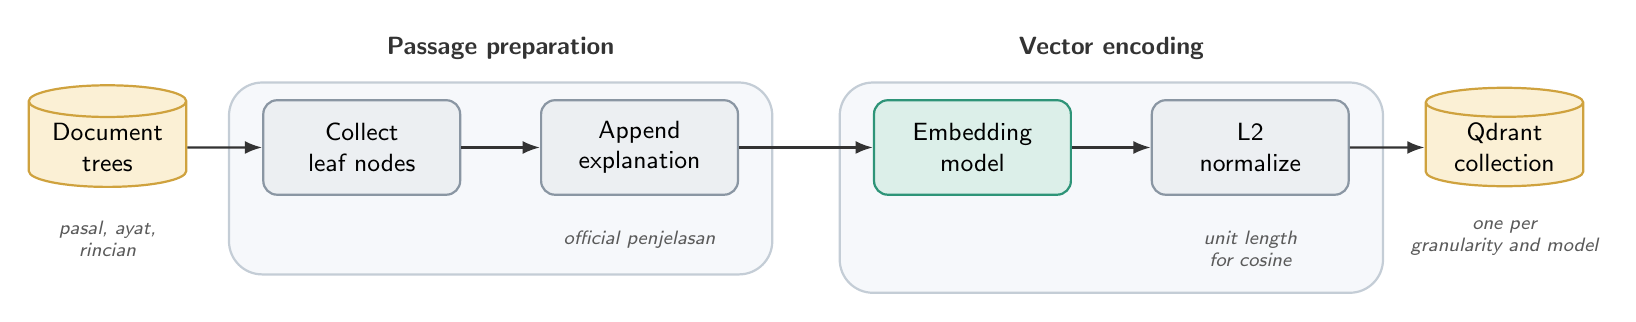
\begin{tikzpicture}

% Source store (outside the phases)
\node[db] (trees) {Document\\trees};

% Phase 1: passage preparation
\node[glue, right=\inlen of trees] (collect) {Collect\\leaf nodes};
\node[glue, right=\intra of collect] (enrich) {Append\\explanation};

% Phase 2: vector encoding
\node[enc, right=\stagegap of enrich] (embed) {Embedding\\model};
\node[glue, right=\intra of embed] (norm) {L2\\normalize};

% Sink store (outside the phases)
\node[db, right=\inlen of norm] (qdrant) {Qdrant\\collection};

% Notes
\node[note, below=0.30cm of trees]  {pasal, ayat,\\rincian};
\node[note, below=0.32cm of enrich] (enrichnote) {official penjelasan};
\node[note, below=0.32cm of norm]   (normnote)   {unit length\\for cosine};
\node[note, below=0.30cm of qdrant] {one per\\granularity and model};

% Phase panels. Source and sink stores stay outside.
\begin{scope}[on background layer]
  \node[region, inner xsep=12pt, inner ysep=6pt,
        fit=(collect)(enrich)(enrichnote)] (reg1) {};
  \node[region, inner xsep=12pt, inner ysep=6pt,
        fit=(embed)(norm)(normnote)] (reg2) {};
\end{scope}
\node[regtitle, anchor=south] at ($(reg1.north)+(0,0.16)$) {Passage preparation};
\node[regtitle, anchor=south] at ($(reg2.north)+(0,0.16)$) {Vector encoding};

% Flow
\draw[flow] (trees)   -- (collect);
\draw[flow] (collect) -- (enrich);
\draw[flow] (enrich)  -- (embed);
\draw[flow] (embed)   -- (norm);
\draw[flow] (norm)    -- (qdrant);

\end{tikzpicture}
\end{document}
